% Options for packages loaded elsewhere
% Options for packages loaded elsewhere
\PassOptionsToPackage{unicode}{hyperref}
\PassOptionsToPackage{hyphens}{url}
%
\documentclass[
  english,
  russian,
  12pt,
  a4paper,
  DIV=11,
  numbers=noendperiod]{scrreprt}
\usepackage{xcolor}
\usepackage{amsmath,amssymb}
\setcounter{secnumdepth}{5}
\usepackage{iftex}
\ifPDFTeX
  \usepackage[T1]{fontenc}
  \usepackage[utf8]{inputenc}
  \usepackage{textcomp} % provide euro and other symbols
\else % if luatex or xetex
  \usepackage{unicode-math} % this also loads fontspec
  \defaultfontfeatures{Scale=MatchLowercase}
  \defaultfontfeatures[\rmfamily]{Ligatures=TeX,Scale=1}
\fi
\usepackage{lmodern}
\ifPDFTeX\else
  % xetex/luatex font selection
\fi
% Use upquote if available, for straight quotes in verbatim environments
\IfFileExists{upquote.sty}{\usepackage{upquote}}{}
\IfFileExists{microtype.sty}{% use microtype if available
  \usepackage[]{microtype}
  \UseMicrotypeSet[protrusion]{basicmath} % disable protrusion for tt fonts
}{}
\usepackage{setspace}
% Make \paragraph and \subparagraph free-standing
\makeatletter
\ifx\paragraph\undefined\else
  \let\oldparagraph\paragraph
  \renewcommand{\paragraph}{
    \@ifstar
      \xxxParagraphStar
      \xxxParagraphNoStar
  }
  \newcommand{\xxxParagraphStar}[1]{\oldparagraph*{#1}\mbox{}}
  \newcommand{\xxxParagraphNoStar}[1]{\oldparagraph{#1}\mbox{}}
\fi
\ifx\subparagraph\undefined\else
  \let\oldsubparagraph\subparagraph
  \renewcommand{\subparagraph}{
    \@ifstar
      \xxxSubParagraphStar
      \xxxSubParagraphNoStar
  }
  \newcommand{\xxxSubParagraphStar}[1]{\oldsubparagraph*{#1}\mbox{}}
  \newcommand{\xxxSubParagraphNoStar}[1]{\oldsubparagraph{#1}\mbox{}}
\fi
\makeatother


\usepackage{longtable,booktabs,array}
\usepackage{calc} % for calculating minipage widths
% Correct order of tables after \paragraph or \subparagraph
\usepackage{etoolbox}
\makeatletter
\patchcmd\longtable{\par}{\if@noskipsec\mbox{}\fi\par}{}{}
\makeatother
% Allow footnotes in longtable head/foot
\IfFileExists{footnotehyper.sty}{\usepackage{footnotehyper}}{\usepackage{footnote}}
\makesavenoteenv{longtable}
\usepackage{graphicx}
\makeatletter
\newsavebox\pandoc@box
\newcommand*\pandocbounded[1]{% scales image to fit in text height/width
  \sbox\pandoc@box{#1}%
  \Gscale@div\@tempa{\textheight}{\dimexpr\ht\pandoc@box+\dp\pandoc@box\relax}%
  \Gscale@div\@tempb{\linewidth}{\wd\pandoc@box}%
  \ifdim\@tempb\p@<\@tempa\p@\let\@tempa\@tempb\fi% select the smaller of both
  \ifdim\@tempa\p@<\p@\scalebox{\@tempa}{\usebox\pandoc@box}%
  \else\usebox{\pandoc@box}%
  \fi%
}
% Set default figure placement to htbp
\def\fps@figure{htbp}
\makeatother



\ifLuaTeX
\usepackage[bidi=basic,provide=*]{babel}
\else
\usepackage[bidi=default,provide=*]{babel}
\fi
% get rid of language-specific shorthands (see #6817):
\let\LanguageShortHands\languageshorthands
\def\languageshorthands#1{}


\setlength{\emergencystretch}{3em} % prevent overfull lines

\providecommand{\tightlist}{%
  \setlength{\itemsep}{0pt}\setlength{\parskip}{0pt}}



 
\usepackage[backend=biber,langhook=extras,autolang=other*]{biblatex}
\addbibresource{bib/cite.bib}

\usepackage[]{csquotes}

\KOMAoption{captions}{tableheading}
\usepackage{indentfirst}
\usepackage{float}
\floatplacement{figure}{H}
\usepackage{libertine}
\makeatletter
\@ifpackageloaded{caption}{}{\usepackage{caption}}
\AtBeginDocument{%
\ifdefined\contentsname
  \renewcommand*\contentsname{Содержание}
\else
  \newcommand\contentsname{Содержание}
\fi
\ifdefined\listfigurename
  \renewcommand*\listfigurename{Список иллюстраций}
\else
  \newcommand\listfigurename{Список иллюстраций}
\fi
\ifdefined\listtablename
  \renewcommand*\listtablename{Список таблиц}
\else
  \newcommand\listtablename{Список таблиц}
\fi
\ifdefined\figurename
  \renewcommand*\figurename{Рисунок}
\else
  \newcommand\figurename{Рисунок}
\fi
\ifdefined\tablename
  \renewcommand*\tablename{Таблица}
\else
  \newcommand\tablename{Таблица}
\fi
}
\@ifpackageloaded{float}{}{\usepackage{float}}
\floatstyle{ruled}
\@ifundefined{c@chapter}{\newfloat{codelisting}{h}{lop}}{\newfloat{codelisting}{h}{lop}[chapter]}
\floatname{codelisting}{Список}
\newcommand*\listoflistings{\listof{codelisting}{Листинги}}
\makeatother
\makeatletter
\makeatother
\makeatletter
\@ifpackageloaded{caption}{}{\usepackage{caption}}
\@ifpackageloaded{subcaption}{}{\usepackage{subcaption}}
\makeatother
\usepackage{bookmark}
\IfFileExists{xurl.sty}{\usepackage{xurl}}{} % add URL line breaks if available
\urlstyle{same}
\hypersetup{
  pdflang={ru-RU},
  hidelinks,
  pdfcreator={LaTeX via pandoc}}


\author{}
\date{}
\begin{document}

\renewcommand*\contentsname{Содержание}
{
\setcounter{tocdepth}{1}
\tableofcontents
}
\listoffigures
\listoftables

\setstretch{1.5}
pdf-engine: xelatex \#\# Author author: name: Никитенко Арина
Александровна degrees: DSc orcid: 0000-0002-0877-7063 email:
1132250435@pfur.ru affiliation: - name: Российский университет дружбы
народов country: Российская Федерация postal-code: 117198 city: Москва
address: ул. Миклухо-Маклая, д. 6

\section{Title}\label{title}

\section{\texorpdfstring{title: \enquote{Лабораторная работа
№2}}{title: ``Лабораторная работа №2''}}\label{title-ux43bux430ux431ux43eux440ux430ux442ux43eux440ux43dux430ux44f-ux440ux430ux431ux43eux442ux430-2}

\chapter{Цель
работы}\label{ux446ux435ux43bux44c-ux440ux430ux431ux43eux442ux44b}

Целью работы является изучение идеологии и применения средств контроля
версий, приобретение практических навыков по работе с системой контроля
версий git.

\#Порядок выполнения работы 1.1 Настройка github Существует несколько
доступных серверов репозиториев с возможностью бесплатного размещения
данных. Например: http://bitbucket.org/, https://github.com/ и
https://gitflic.ru. Для выполнения лабораторных работ предлагается
использовать Github. Создайте учётную запись на сайте
https://github.com/ и заполните основные данные (рис.~\ref{fig-001}).

\begin{figure}

\centering{

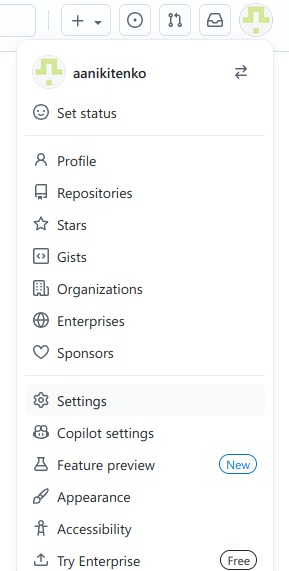
\includegraphics[width=0.7\linewidth,height=\textheight,keepaspectratio]{image/1.png}

}

\caption{\label{fig-001}Создание профиля в github}

\end{figure}%

1.2. Базовая настройка git Сначала сделаем предварительную конфигурацию
git. Откроем терминал и введем следующие команды, указав имя и e-mail
владельца репозитория:

git config --global user.name \enquote{} git config --global user.email
\enquote{\href{mailto:work@mail}{\nolinkurl{work@mail}}}

(рис.~\ref{fig-002}).

\begin{figure}

\centering{

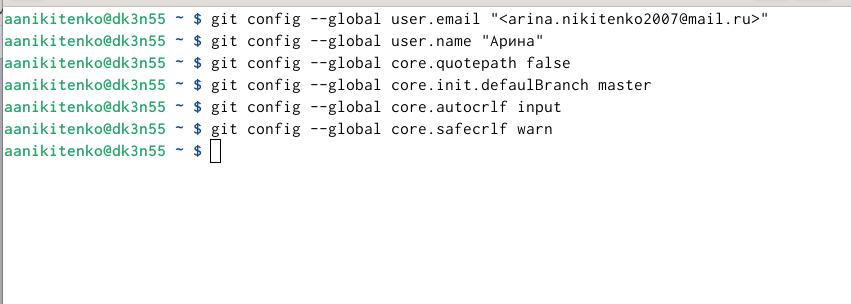
\includegraphics[width=0.7\linewidth,height=\textheight,keepaspectratio]{image/2.png}

}

\caption{\label{fig-002}Предварительная настройка git}

\end{figure}%

Настроим utf-8 в выводе сообщений git: git config --global
core.quotepath false Зададим имя начальной ветки (будем называть её
master): git config --global init.defaultBranch master

Параметр autocrlf: git config --global core.autocrlf input

Параметр safecrlf: git config --global core.safecrlf warn

1.3 Создание SSH-ключа

Для последующей идентификации пользователя на сервере репозиториев
сгенерируем ключ: (рис.~\ref{fig-003}).

\begin{figure}

\centering{

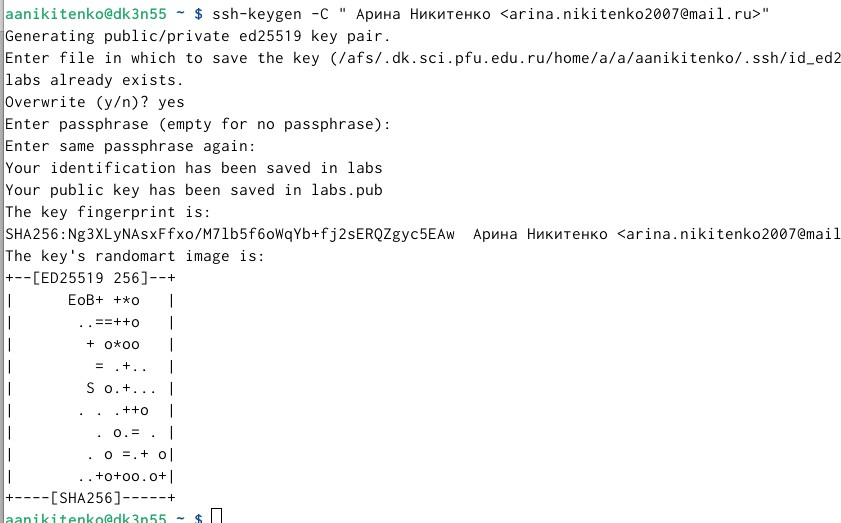
\includegraphics[width=0.7\linewidth,height=\textheight,keepaspectratio]{image/3.png}

}

\caption{\label{fig-003}Создание ключа}

\end{figure}%

(рис.~\ref{fig-004}).

\begin{figure}

\centering{

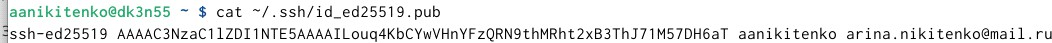
\includegraphics[width=0.7\linewidth,height=\textheight,keepaspectratio]{image/4.png}

}

\caption{\label{fig-004}Создание ключа}

\end{figure}%

Далее нам необходимо загрузить сгенерированный ключ. Для этого зайдем на
сайт http://github.org/ под своей учётной записью и перейдем в меню
Setting . После этого выберем в боковом меню SSH and GPG keys и нажмем
кнопку New SSH key . Копируем из локальной консоли ключ в буфер обмена,
и вставляем ключ в появившееся на сайте поле, и указываем для ключа имя
(key) :

(рис.~\ref{fig-005}).

\begin{figure}

\centering{


\includegraphics[width=0.7\linewidth,height=\textheight,keepaspectratio]{image/5.png}

}

\caption{\label{fig-005}Ключ}

\end{figure}%

1.4. Создание рабочего пространства и репозитория курса

При выполнении лабораторных работ следует придерживаться структуры
рабочего пространства. Откроем терминал и создадим каталог для предмета
«Архитектура компьютера» (рис.~\ref{fig-006}).

\begin{figure}

\centering{


\includegraphics[width=0.7\linewidth,height=\textheight,keepaspectratio]{image/6.png}

}

\caption{\label{fig-006}Создание каталога для «Архитектура компьютера»}

\end{figure}%

1.5. Создание репозитория курса

Репозиторий на основе шаблона можно создать через web-интерфейс github.
Перейдем на станицу репозитория с шаблоном курса
https://github.com/yamadharma/cour se-directory-student-template и далее
выберите Use this template : (рис.~\ref{fig-007}).

\begin{figure}

\centering{

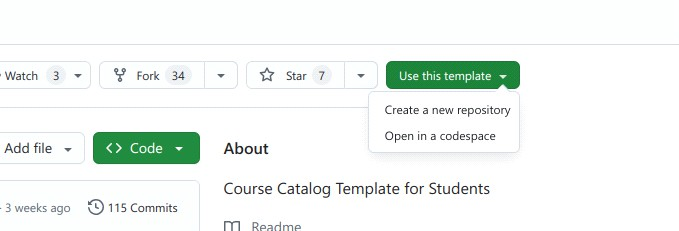
\includegraphics[width=0.7\linewidth,height=\textheight,keepaspectratio]{image/7.png}

}

\caption{\label{fig-007}Use this template}

\end{figure}%

В открывшемся окне зададим имя репозитория (Repository name)
study\_2025-- 2026\_arh-pc и создадим репозиторий (кнопка Create
repository from template):

(рис.~\ref{fig-008}).

\begin{figure}

\centering{

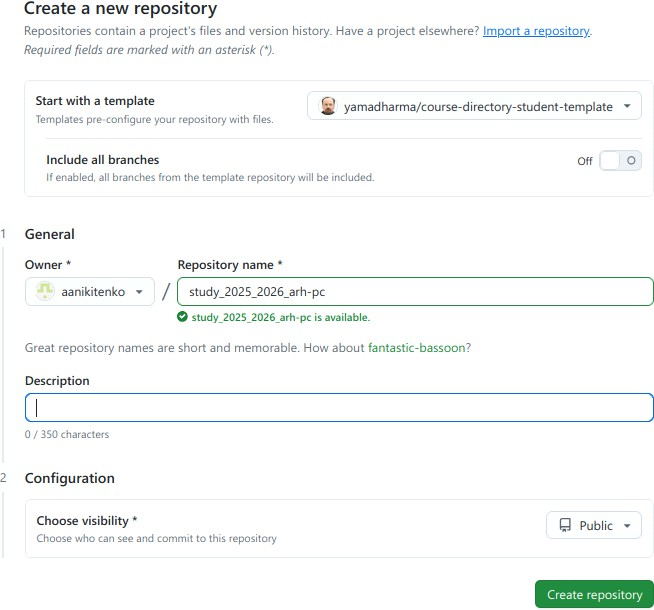
\includegraphics[width=0.7\linewidth,height=\textheight,keepaspectratio]{image/8.png}

}

\caption{\label{fig-008}Создание репозитория}

\end{figure}%

Ссылку для клонирования можно скопировать на странице созданного
репозитория Code -\textgreater{} SSH:

(рис.~\ref{fig-009}).

\begin{figure}

\centering{

\includegraphics[width=0.7\linewidth,height=\textheight,keepaspectratio]{image/0.png}

}

\caption{\label{fig-009}Копирование репозитория}

\end{figure}%

Клонируем созданный репозиторий:

(рис.~\ref{fig-010}).

\begin{figure}

\centering{

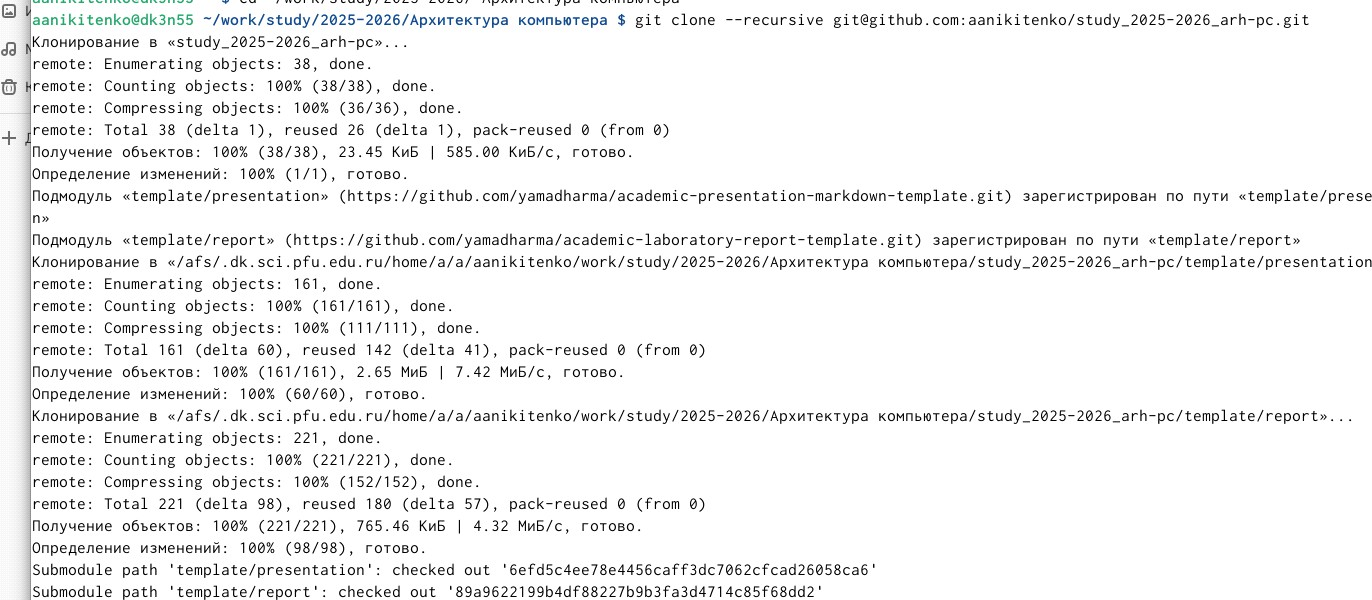
\includegraphics[width=0.7\linewidth,height=\textheight,keepaspectratio]{image/10.png}

}

\caption{\label{fig-010}Клонирование репозитория}

\end{figure}%

(рис.~\ref{fig-011}).

\begin{figure}

\centering{

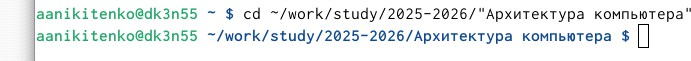
\includegraphics[width=0.7\linewidth,height=\textheight,keepaspectratio]{image/11.png}

}

\caption{\label{fig-011}Переход в каталог курса}

\end{figure}%

1.6. Настройка каталога курса

Выполним следующие действия : 1) перейдем в каталог курса и создадим
необходимые каталоги: echo arch-pc \textgreater{} COURSE make prepare 2)
отправим файлы на сервер: git add . git commit -am \enquote*{feat(main):
make course structure} git push (рис.~\ref{fig-012}).

\begin{figure}

\centering{

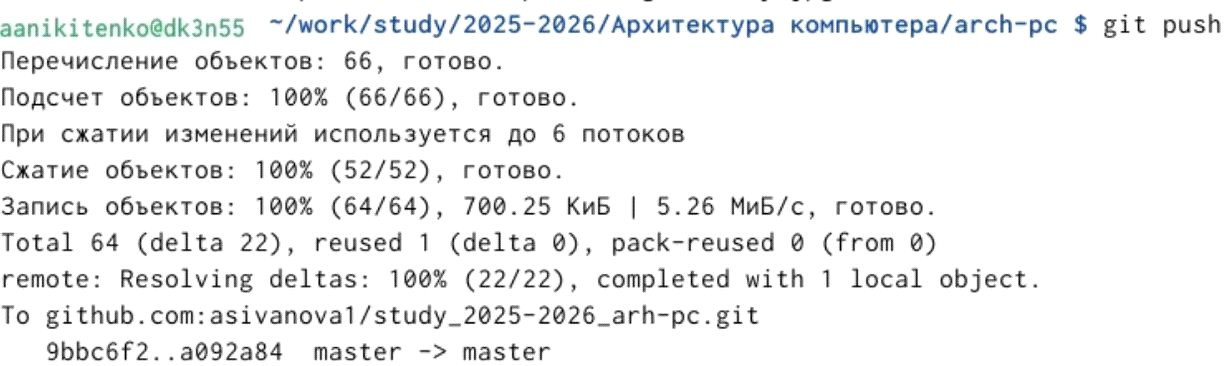
\includegraphics[width=0.7\linewidth,height=\textheight,keepaspectratio]{image/12.png}

}

\caption{\label{fig-012}Выполнение команд}

\end{figure}%

(рис.~\ref{fig-013}).

\begin{figure}

\centering{

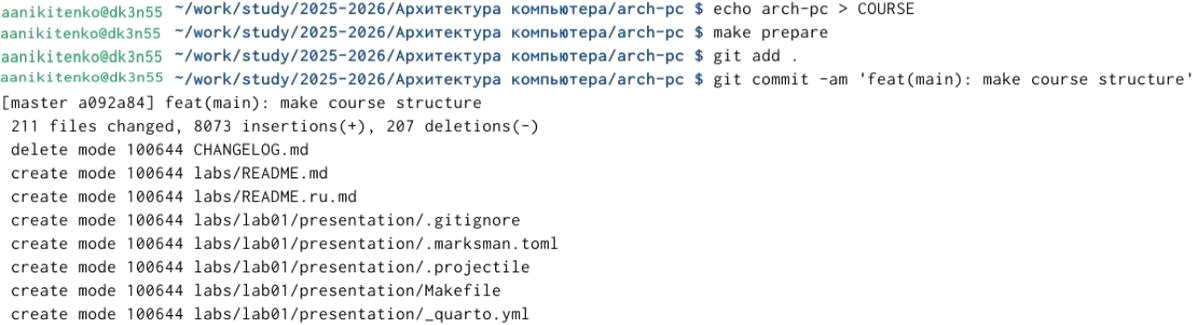
\includegraphics[width=0.7\linewidth,height=\textheight,keepaspectratio]{image/13.png}

}

\caption{\label{fig-013}Выполнение команд}

\end{figure}%

\chapter{2.Задания для самостоятельной
работы}\label{ux437ux430ux434ux430ux43dux438ux44f-ux434ux43bux44f-ux441ux430ux43cux43eux441ux442ux43eux44fux442ux435ux43bux44cux43dux43eux439-ux440ux430ux431ux43eux442ux44b}

\begin{enumerate}
\def\labelenumi{\arabic{enumi}.}
\tightlist
\item
  Создадим отчет по выполнению лабораторной работы в соответствующем
  каталоге рабочего пространства (labs/lab02/report):
  (рис.~\ref{fig-014}).
\end{enumerate}

\begin{figure}

\centering{

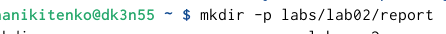
\includegraphics[width=0.7\linewidth,height=\textheight,keepaspectratio]{image/14.png}

}

\caption{\label{fig-014}}

\end{figure}%

\chapter{Вывод}\label{ux432ux44bux432ux43eux434}

Мы изучили идеологию и применение средств контроля версий, а также
приобрели практические навыки по работе с системой контроля версий git.

\printbibliography[heading=none]





\end{document}
